\documentclass[answers]{exam}

%% Language and font encodings
\usepackage[english]{babel}
\usepackage[utf8x]{inputenc}
\usepackage[T1]{fontenc}
% \usepackage{enumitem}
%% Sets page size and margins
\usepackage[a4paper,margin=2cm]{geometry}

%% Useful packages
\usepackage[font=small,labelfont=bf]{caption}
\usepackage{amsmath}
\usepackage{amssymb}
\usepackage{graphicx}
\usepackage{paralist}
\usepackage{framed}
\usepackage{tikz}
\usepackage{float}
\usepackage{listings}
\usepackage{xcolor}
\tikzset{
  % define the bar graph element
  bar/.pic={
    \fill (-.1,0) rectangle (.1,#1) (0,#1) node[above,scale=1/2]{$#1$};
  }
}
\definecolor{codegreen}{rgb}{0,0.6,0}
\definecolor{codegray}{rgb}{0.5,0.5,0.5}
\definecolor{codepurple}{rgb}{0.58,0,0.82}
\definecolor{backcolour}{rgb}{0.95,0.95,0.92}
% Colored Python listing from https://www.overleaf.com/learn/latex/Code_listing
\definecolor{codegreen}{rgb}{0,0.6,0}
\definecolor{codegray}{rgb}{0.5,0.5,0.5}
\definecolor{codepurple}{rgb}{0.58,0,0.82}
\definecolor{backcolour}{rgb}{0.95,0.95,0.92}
 
\lstdefinestyle{mystyle}{
    backgroundcolor=\color{backcolour},   
    commentstyle=\color{codegreen},
    keywordstyle=\color{magenta},
    numberstyle=\tiny\color{codegray},
    stringstyle=\color{codepurple},
    basicstyle=\ttfamily\footnotesize,
    breakatwhitespace=false,         
    breaklines=true,                 
    captionpos=b,                    
    keepspaces=true,                 
    numbers=left,                    
    numbersep=5pt,                  
    showspaces=false,                
    showstringspaces=false,
    showtabs=false,                  
    tabsize=2
}
\lstset{style=mystyle}

\usetikzlibrary{matrix}

\setlength\FrameSep{4pt}
\title{Probability \& Statistics\\ Project}
\author{Hana Ali Rashid, hr05940\\ Tasmiya Malik, tm06183\\ Ifrah Ilyas, ii06178}
\date{\today{}}
\begin{document}
\maketitle

% \noindent \hrulefill \\
% \textbf{Instructions:}
% \begin{itemize}
%     \item \textbf{Pairs can not be cross-section.}
% \end{itemize}

% \noindent \hrulefill

\section*{Q1: Random Walk}
\subsection*{1.1}
Function implementation in Python:
\lstinputlisting[firstline=5,lastline=13,language=python]{q1.py}
Calling the function for several iterations to get multiple expected values:
\lstinputlisting[firstline=16,lastline=33,language=python]{q1.py}
\pagebreak
Histograms produced by the above code for various combinations of $n$ and $p$:\\
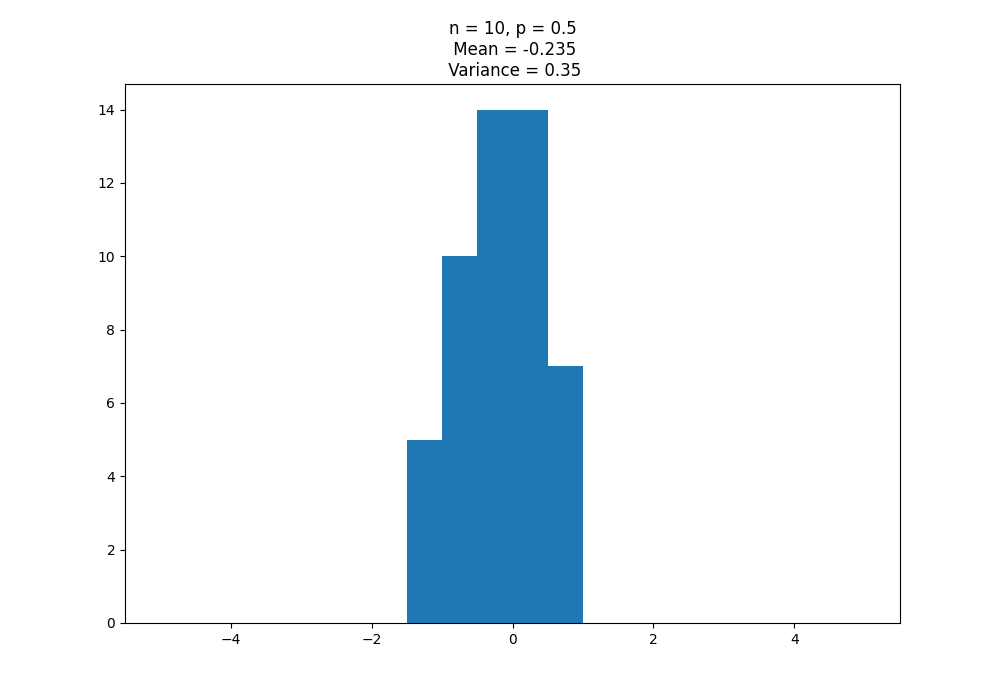
\includegraphics[scale = 0.5]{Q1_histograms/1.1/q1_n = 10_ p = 0.5.png}\\
The above histogram appears to follow a normal distribution with a mean of $3.267$ and variance of $0.233$.\\
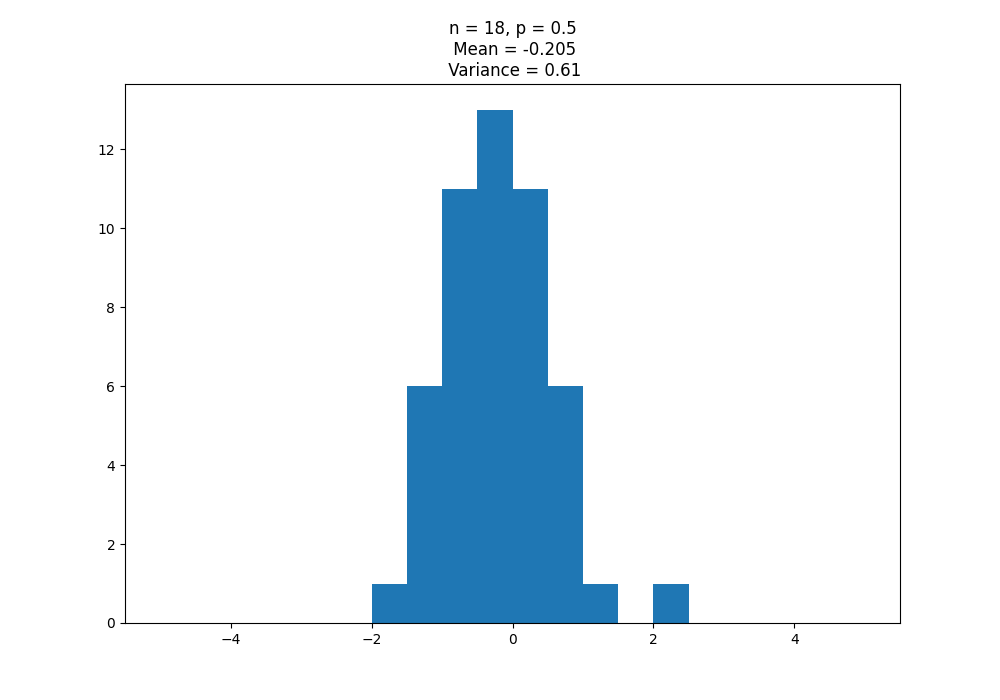
\includegraphics[scale = 0.5]{Q1_histograms/1.1/q1_n = 18_ p = 0.5.png}\\
The above histogram appears to follow a normal distribution with a mean of $3.267$ and variance of $0.233$.\\
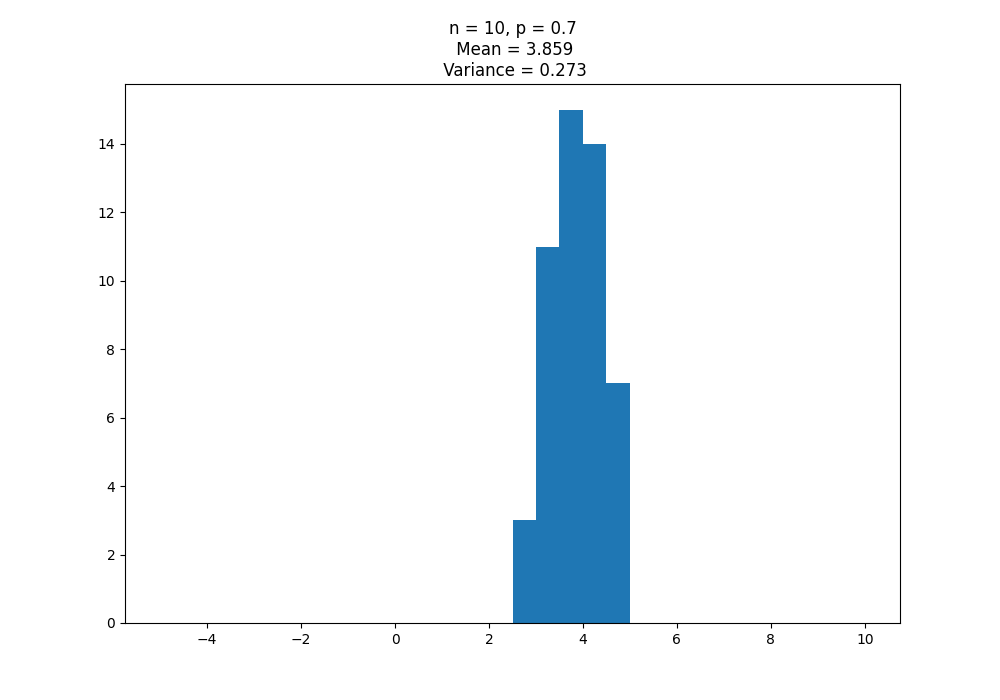
\includegraphics[scale = 0.5]{Q1_histograms/1.1/q1_n = 10_ p = 0.7.png}\\
The above histogram appears to follow a normal distribution with a mean of $3.267$ and variance of $0.233$.\\
\pagebreak
%--------------------------------  1.2  ------------------------------------
\subsection*{1.2}
Function implementation in Python:
\lstinputlisting[firstline=36,lastline=44,language=python]{q1.py}
Calling the function for several iterations to get multiple expected values:
\lstinputlisting[firstline=46,lastline=63,language=python]{q1.py}
\pagebreak
Histograms produced by the above code for various combinations of $n$ and $p$:\\
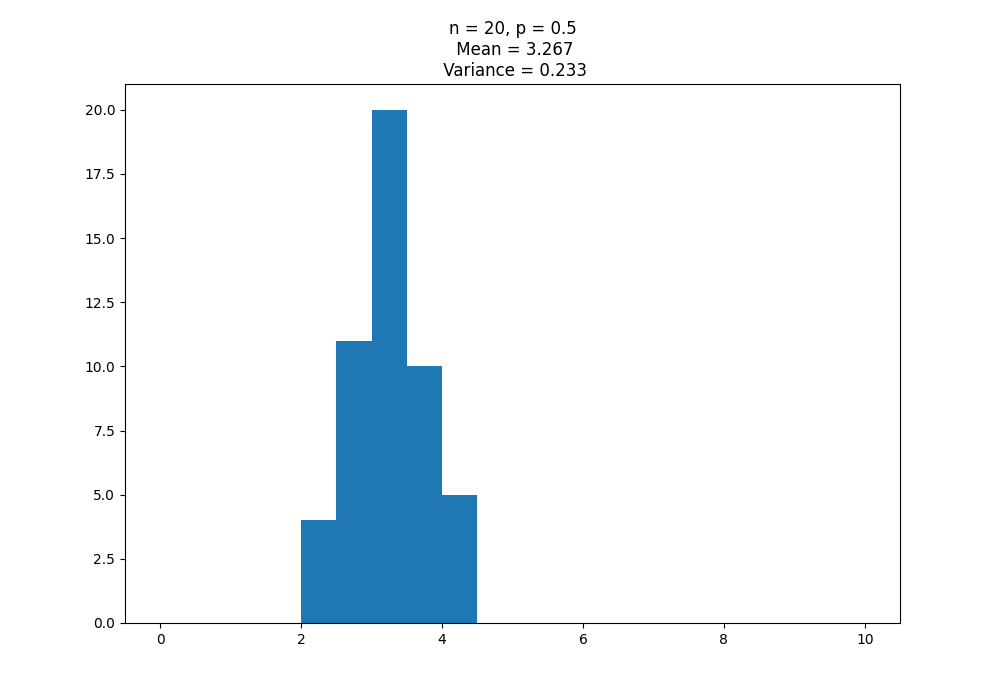
\includegraphics[scale = 0.5]{Q1_histograms/1.2/Q1.2 _n = 20_p = 0.5.png}\\
The above histogram appears to follow a normal distribution with a mean of $3.267$ and variance of $0.233$.\\
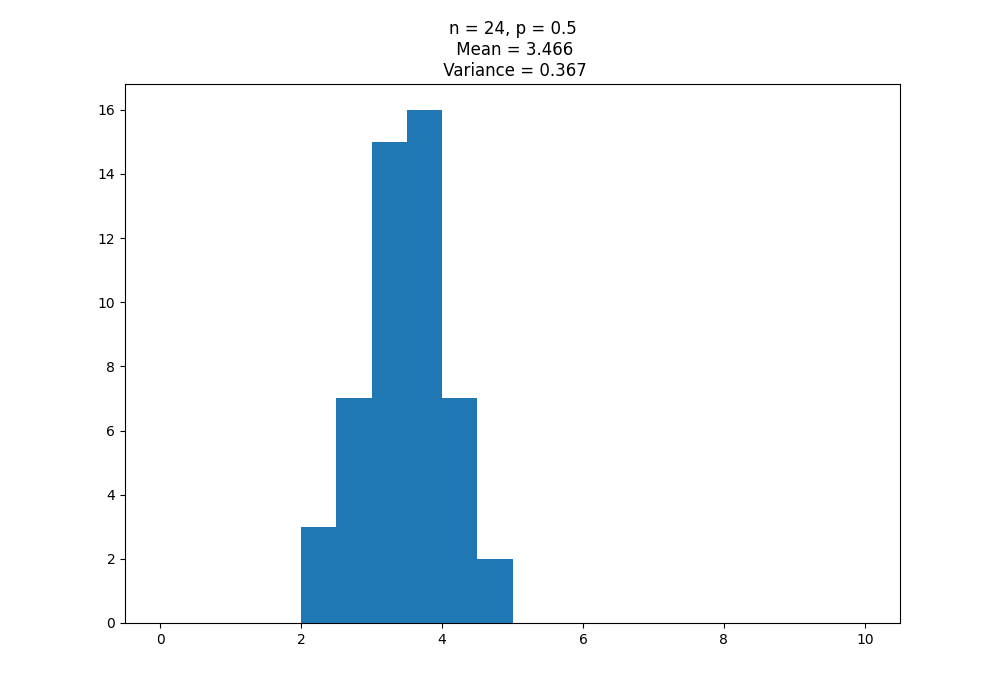
\includegraphics[scale = 0.5]{Q1_histograms/1.2/Q1.2 _n = 24_p = 0.5.png}\\
The above histogram shows that...\\
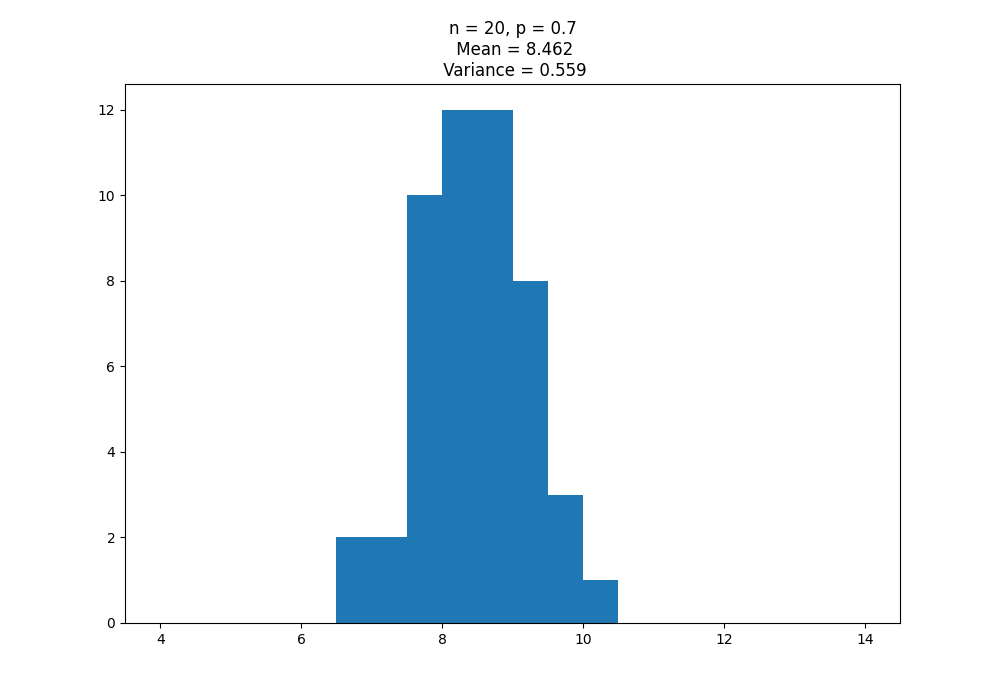
\includegraphics[scale = 0.5]{Q1_histograms/1.2/Q1.2 _n = 20_p = 0.7.png}\\
The above histogram shows that...\\
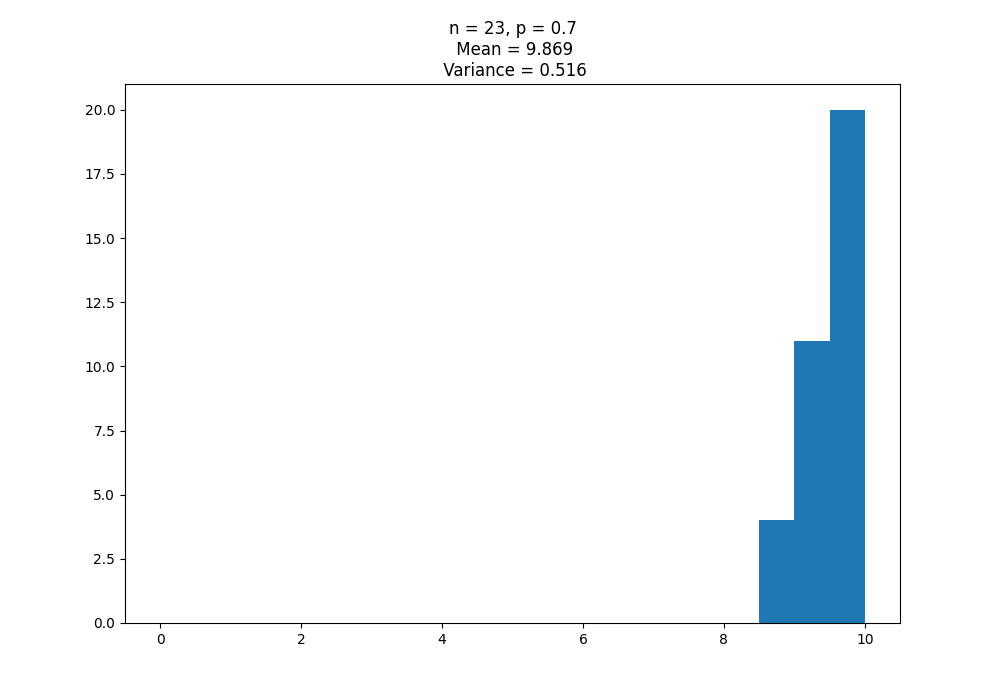
\includegraphics[scale = 0.5]{Q1_histograms/1.2/Q1.2 _n = 23_p = 0.7.png}

\pagebreak
%--------------------------------  1.3  ------------------------------------
\subsection*{1.3}
Function implementation in Python:
\lstinputlisting[firstline=65,lastline=79,language=python]{q1.py}
Calling the function for several iterations to get multiple expected values:
\lstinputlisting[firstline=81,lastline=104,language=python]{q1.py}
\newpage
%--------------------------------  2.*  ------------------------------------
\section*{Q2: Simulating Distributions}

%--------------------------------  2.1  ------------------------------------
  \subsection*{2.1}
        It does accomplish as it plots for a value of x (y is the variable expressed in terms of x) against the pdf $e^{-y}$ such that each bar in the histogram shows the probability for an average value of x. The distrubution plotted is a continuous exponential random variable. The number of bins used are significant for our simulation which will become evident with the following images:
        \begin{center}
          \begin{tabular}{cc}
            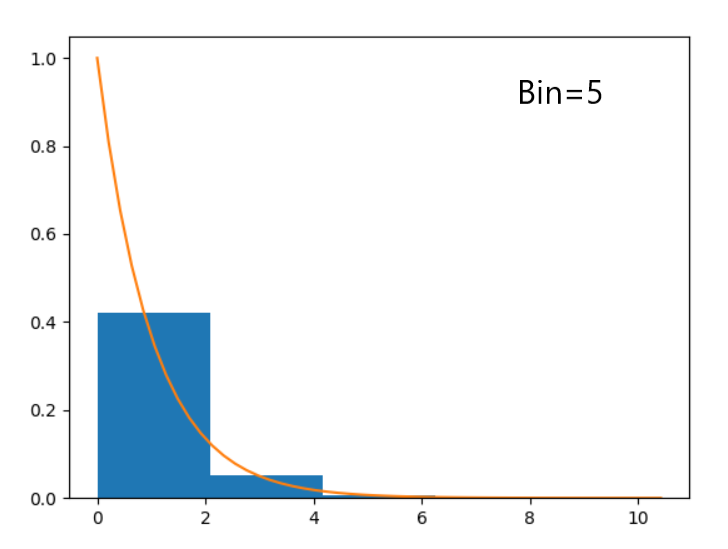
\includegraphics[width= 0.35\textwidth]{"Q2/bin5.png"}
            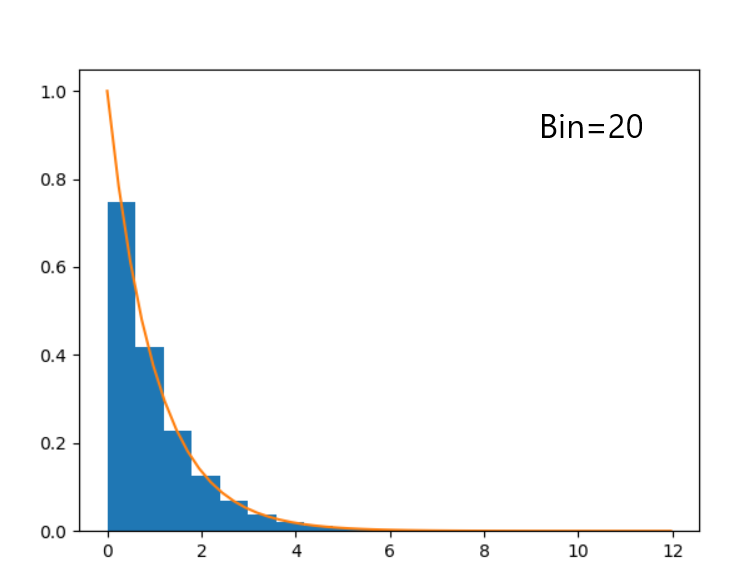
\includegraphics[width= 0.36\textwidth]{"Q2/bin20.png"}\\
            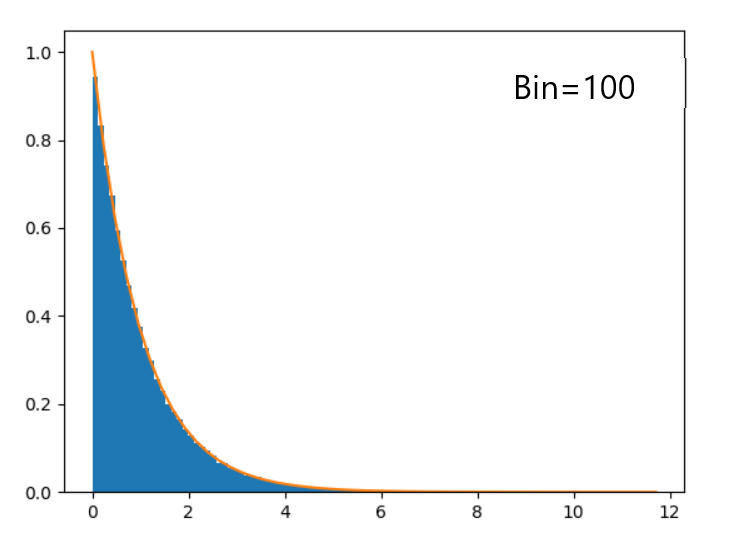
\includegraphics[width= 0.375\textwidth]{"Q2/bin100.png"}
            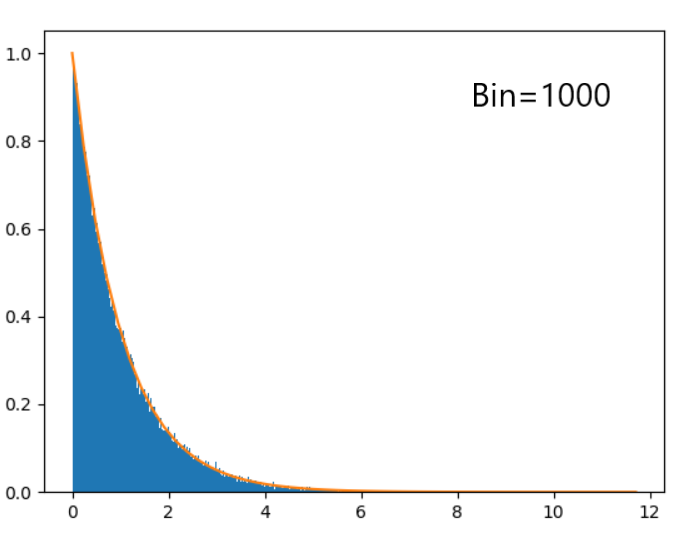
\includegraphics[width= 0.35\textwidth]{"Q2/bin1000.png"}    
          \end{tabular}
          \captionof{figure}{Simulations done with different number of bins} 
        
       
      \end{center} 
      It is noticeable that, with more number of bins, the accuracy of the results increases. However, it is also interesting to note that using 1000 bins almost gives the same result as 100 bins. Therefore, while simulating we need to take an appropriate values for bins for better approximation and less running time.

%--------------------------------  2.2  ------------------------------------
  \subsection*{2.2}  
      In the code we see that :
         $$y=\frac{1}{1-x} $$
         With the trick shown, we can back track to find the original distribution.
        $$1-\frac{1}{y}=x $$
        We know that the upper bound will be y. For the lower bound we see that:
        $$\frac{1}{1}-\frac{1}{y}=x $$
        $$-(\frac{1}{y}-\frac{1}{1})=x $$
        $$\therefore - \frac{1}{y}\Biggr|^{y}_{1}=x $$
        Performing derivative on the left hand side:
        $$\frac{d}{dy} \frac{-1}{y}=(-1)\frac{-1}{y^2}=\frac{1}{y^2}$$
        $$\therefore \int_{1}^{y} \frac{1}{y^2} dy=x$$
        We can affirm that we have reached the right deduction by looking at line 12 of the code.
        So, the distribution of y is :
        $$f_Y(y)=\frac{1}{y^2} for y \geq 1$$
         \lstinputlisting[firstline=23,lastline=25,language=python]{Q2.py}
        Lines 5-7 is simply trying to implement a cutoff for values of y greater 30 as values starting to get more smaller. Given that we taken small amount of bins, the average value of each bar becomes negligible and is not visible in the graph. Therefore we cut it down to 30 so that the approximation is more accurate.
     \begin{center}
      \begin{tabular}{cc}
      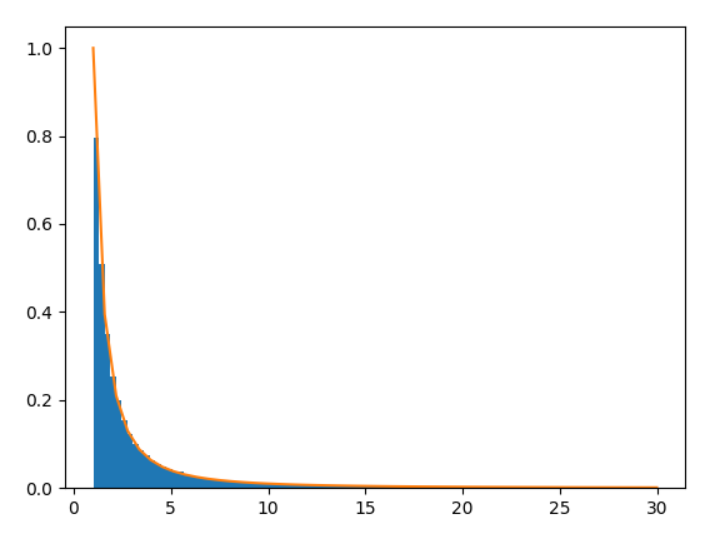
\includegraphics[width= 0.4\textwidth]{"Q2/beforeremoving.png"}
    \end{tabular}
    \captionof{figure}{Before Removing} 
    \begin{tabular}{cc}
      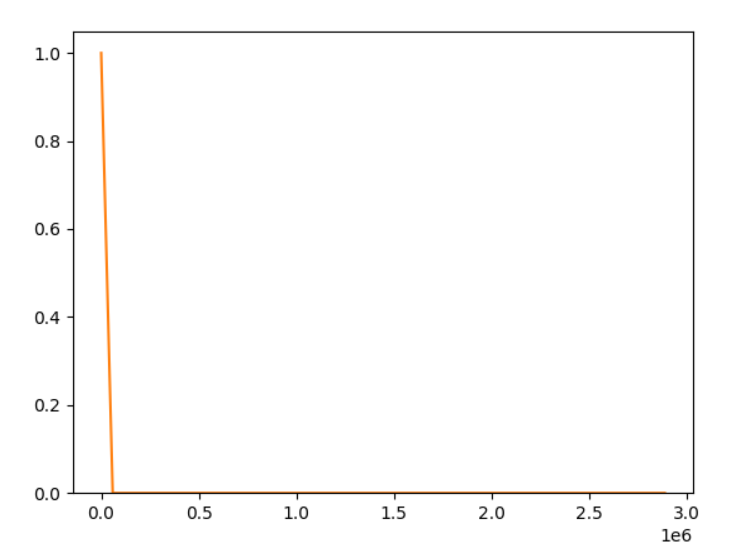
\includegraphics[width= 0.4\textwidth]{"Q2/afterremoving.png"}
      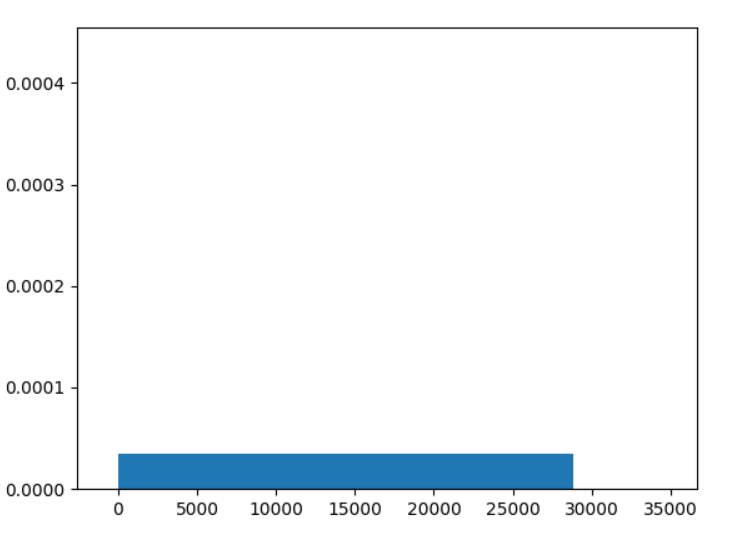
\includegraphics[width= 0.4\textwidth]{"Q2/afterremoving2.png"} 
    \end{tabular} 
    \captionof{figure}{After Removing} 
    \end{center}
        
%--------------------------------  2.3  ------------------------------------
  \subsection*{2.3}    
    For, $$f_Y (y) = \frac{1}{y^3}
        for y \geq \sqrt{\frac{1}{2}}$$
         $$ P(Y<y)=P(X<x)$$
         $$\int_{\sqrt{\frac{1}{2}}}^{y} \frac{1}{y^3} dy=x$$
         $$ \frac{-1}{2y^2} \Biggr|^{y}_{\sqrt{\frac{1}{2}}}=x$$
         $$ \frac{-1}{2y^2} +\frac{1}{2(\sqrt{\frac{1}{2}})^2}=x$$
         $$ \frac{-1}{2y^2} +1=x$$
         $$ \frac{1}{2y^2} =1-x$$
         $$ y^2=\frac{1}{2(1-x)}$$
         $$ y=\sqrt{\frac{1}{2(1-x)} }$$
         Code:
         \lstinputlisting[firstline=35,lastline=48,language=python]{Q2.py}
         The output of simulation for this y:
         \begin{center}
          \begin{tabular}{cc}
          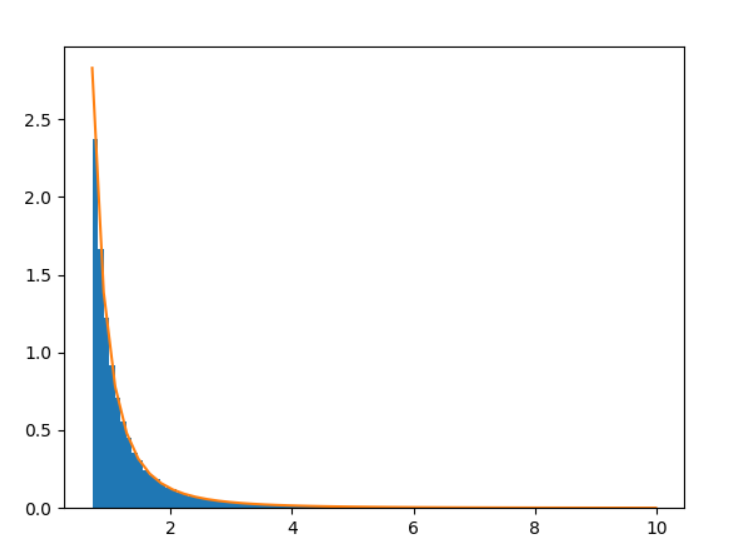
\includegraphics[width= 0.4\textwidth]{"Q2/2.3.png"}
        \end{tabular}
        \captionof{figure}{Simulation of distribution $f_Y (y) = \frac{1}{y^3}
        for y \geq \sqrt{\frac{1}{2}}$} 
      \end{center}
      For the simulation of expected values, the same code used for the above function ran for 10000 times and each run would take the mean of y :
         \lstinputlisting[firstline=51,lastline=62,language=python]{Q2.py}
      The output of this simulation:
         \begin{center}
        \begin{tabular}{cc}
        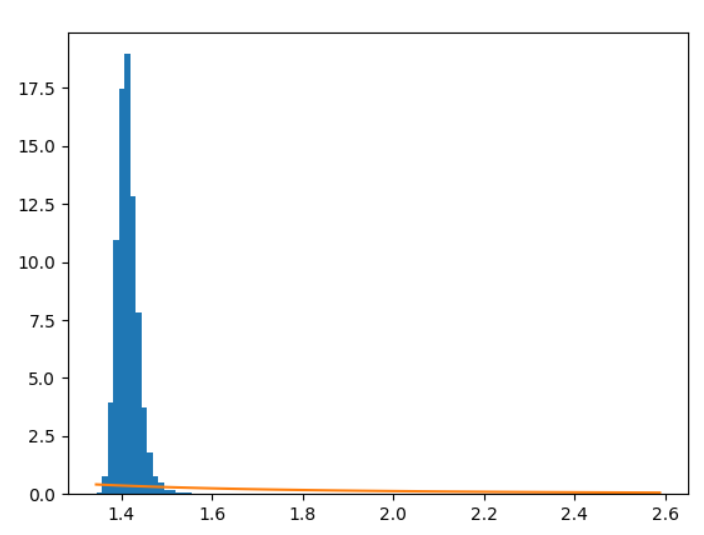
\includegraphics[width= 0.4\textwidth]{"Q2/expected value.png"}
      \end{tabular}
      \captionof{figure}{Simulation of expected values of $fY (y) = \frac{1}{y^3}
      for y \geq \sqrt{\frac{1}{2}}$} 
    \end{center}


%--------------------------------  3.*  ------------------------------------
\section*{Q3. Picking a Random Point Correctly}

\subsection*{3.1}

\begin{framed}
  For part $3.1$, we followed the method specified in the question. The program takes radius as an input from the user, and passes it to \emph{gen\_points(R)} to display the graph. It first finds random radius R and angle $\theta$, then converts it into cartesian cordinates. It stores the values of x and y till the iterations are running, then plot the points. To make sure the points lie in the given radius, we also draw the circle.
  \begin{itemize}
    \item \emph{polar\_to\_cart(r,t)}: This function takes the polar cordinates $(r \;\text{and}\; \theta)$ and converts them to their cartesian equivalent. It is called from \emph{random\_point(R)}, to return the cartesian cordinates. It uses the following formulae,\\
      \begin{align*}
        x &= r\cos(\theta)\\
        y &= r\sin(\theta)
      \end{align*}

    \item \emph{random\_point(R)}: The function is responsible for generating a random point in polar cordinates, and returns the converted cartesian cordinates.\\
    
    \item \emph{gen\_points(R)}: This is the main function which runs 1000 iterations, and calls \emph{random\_point(R)}, and stores the result in the separate lists for $X$ and $Y$ cordinates. Then the lists are passed to the plot functions, to graph the points.

  \end{itemize}
  The resulting graph has very dense distribution towards the center.
\end{framed}

\lstinputlisting[firstline=1,lastline=48,language=python]{Q3/Q3(1).py}

\begin{figure}[h]
  \centering
  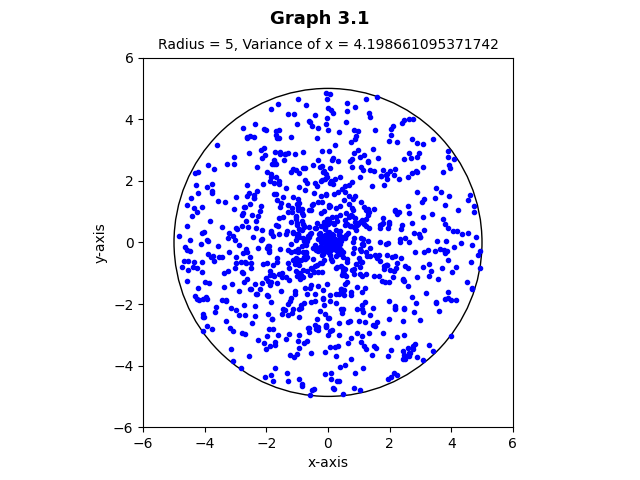
\includegraphics[scale=0.7]{Q3/Q3(1).png}
\end{figure}
\newpage
%--------------------------------  3.2  ------------------------------------
\subsection*{3.2}
\begin{framed}
  \indent In part $3.2$, we calculated the cartesian cordinates directly from the specified radius R. If the random point lied farther from the distance from the origin, it will be discarded and the program will find a new point.
  \begin{itemize}
    \item \emph{random\_point(R)}: This function finds random points for $x$ and $y$ cordinates between the range $-R$ and $R$. It returns the tuple with cartesian cordinates.\\
    
    \item \emph{dist\_from\_origin(x,y)}: The function find and return the distance of the point from the origin.\\
      \begin{align*}
        dist=\sqrt{x^2+y^2}
      \end{align*}
    \item \emph{gen\_points(R)}: The main function iterates 1000 times and calls \emph{random\_point(R)}. Then it checks the condition that if the distance of the point $(x,y)$ is within the radius $R$, it would append the points to their respective lists, else the counter will be decremented by 1 and the point will not be added to the list. Then the lists $X$ and $Y$ are passed to the plot functions for display.
  \end{itemize}
\end{framed}
\lstinputlisting[firstline=1,lastline=46,language=python]{Q3/Q3(2).py}
\begin{figure}[h]
  \centering
  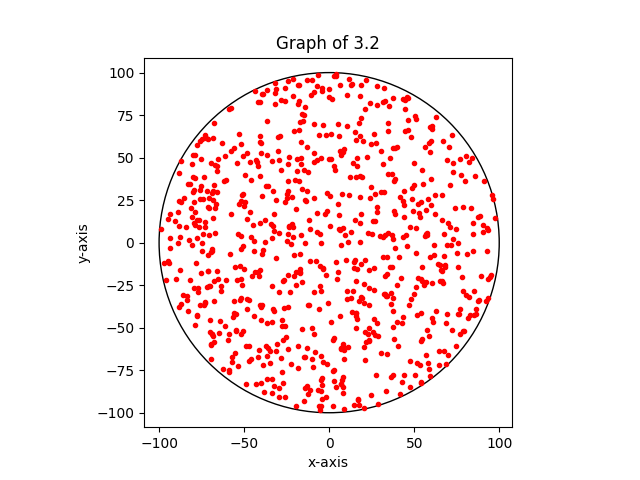
\includegraphics[scale=0.7]{Q3/Q3(2).png}
\end{figure}
\newpage
%--------------------------------  3.3  ------------------------------------
\subsection*{3.3}
\begin{framed}
  \indent In part $3.3$, we had to modify the function for polar cordinates, such that the graph it made was uniformly distributed, similar to the histogram of part $3.2$.\\
  \indent The reason behind the uneven distribution when we used polar cordinates was because of the way polar and cartesian planes interact. If we plot points in a smaller radius with varying angles, the points will be closer, as compare to a larger radius. For larger radius the points will be far apart. So when we were converting them into cartesian cordinates, many of them lied near the origin. To solve this, we simply take the CDF, i.e. the area of the circle, and make radius r its subject. Mathematically,\\
  \begin{align*}
    P(r\leq R)&=k.\pi.r^2\\
    \intertext{To find k, we use P(r=R), which is equals to 1.}\\
    k.\pi.R^2&=1\\
    k &= \frac{1}{R^2\pi}\\
    \intertext{Now that we know the value of k, we can find the whole CDF by plugging its value.}\\
    CDF &= (\frac{1}{R^2\pi})(r^2\pi)=\frac{r^2}{R^2}\\
    \intertext{Now we make radius r, the subject of the equation.}\\
    r &= \sqrt{R^2.CDF} = R\sqrt{CDF}
  \end{align*}
  \indent We can find our random radius r using this formula. This will produce the points in proportionality with the area of the circle, thus keeping the point uniform.\\
  \indent From here, we will describe the functionality of the coded program.

  \begin{itemize}
    \item \emph{random\_point(R)}: The function finds random radius R and theta $\theta$. It uses the function for R derived above. 

    \item \emph{polar\_to\_cart(cord)}: This is the same function that we used in part 3.1. The function takes radius r and angle t as the input, and returns the cartesian cordinates. We use the following formulae to derive the cordinates,\\
      \begin{align*}
        x &= r\cos(t)\\
        y &= r\sin(t)
      \end{align*}
    \item \emph{gen\_points(R)}: Like previous parts, this function makes 1000 iterations, and call \emph{random\_point(R)} for each of them, then stores the returned values in their respective lists X and Y.\\
      Then it draws outer and inner circles of the given radius R and $\frac{R}{2}$ respectively, and then plot the points stored in the lists X and Y.
  \end{itemize}
\end{framed}
\lstinputlisting[firstline=1,lastline=53,language=python]{Q3/Q3(3).py}

\begin{figure}[h]
  \centering
  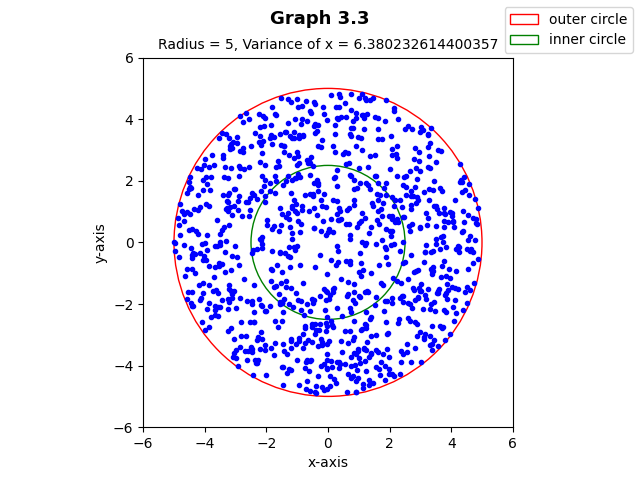
\includegraphics[scale=0.7]{Q3/Q3(3).png}
\end{figure}
\newpage

\section*{Q4. Saying Random is not enough}

%--------------------------------  4.1  ------------------------------------
  \subsection*{4.1}
    \begin{framed}
        For 4.1, we took the approach specified in the question. We first pick two random angles $\theta_1$ and $\theta_2$. Then find their difference to find the angle lying in between $\theta_1$ and $\theta_2$. Then we use this new angle in \emph{cord length} formula. The program does this process 1000 times and stores the values in the specified list, then graphs a histogram for the length of the cords and the probability of them occuring. Following describes each function and their purpose/method for the program.
        \begin{enumerate}
            \item \emph{random\_theta()}: The function finds random $\theta_1$ and $\theta_2$. $\theta$ is chosen randomly from degrees($\phi$) and then converted to radians.
                    \begin{align*}
                        \theta_1 &= \phi_1 . \frac{\pi}{180}\\
                        \theta_2 &= \phi_2 . \frac{\pi}{180}
                    \end{align*}
            \item \emph{cord(R)}: The function takes the radius as the input and returns length of the cord between $\theta_1$ and $\theta_2$. It first calls \emph{random\_theta()}, and find the absolute value of their difference ($\theta=|\theta_1 - \theta_2|$). Then the length of the cord in calculated using the following formula for cord length,
                    $$\text{cord length}=2R.\sin(\theta/2)$$
            \item \emph{find\_cords1(R)}: The function takes radius R as input, then draw the histogram as the output. It iterates 1000 times, calls \emph{cord(R)} for each iteration and append the result in \emph{cord\_len}. The bin value is set to be 50 as it provides a good threshold for the 1000 values. Then it plots the graph using matplotlib.
        \end{enumerate}
    \end{framed}
    \lstinputlisting[firstline=5,lastline=34,language=python]{Q4.py}
    \begin{figure}[ht]
        \caption{Histogram of 4.1}
        \centering
        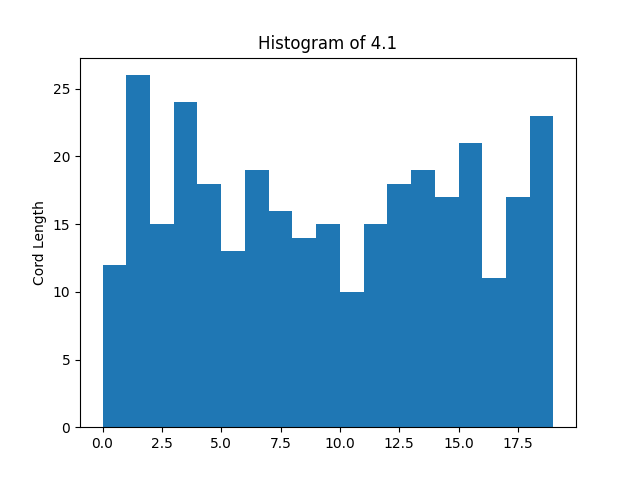
\includegraphics[scale=0.7]{Q4/Q4(1).png}
    \end{figure}
\newpage
%--------------------------------  4.2  ------------------------------------
  \subsection*{4.2}
    \begin{framed}
        For 4.2, we follow the instructions given in the question. We first pick a direction/angle and assume an imaginary radius there. Then we pick a random point on that radius and find its distance from the origin $(0,0)$. This serves as our base, while to radius R serves as our hypotaneous. Then we find the perpendicular using the pythagorean theorem, and returns the twice of it. As the perpendicular shows the half part of that cord, with randomly chosen point as its center. This point is also the midpoint for our circle, so we double the perpendicular to find the whole cord length.
        \begin{center}
            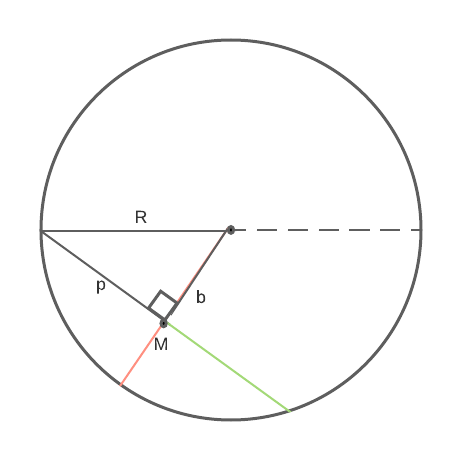
\includegraphics[scale=0.7]{Q4/4.2_circle.png}
        \end{center}
        \begin{enumerate}
            \item \emph{random\_cord(R)}: This function does multiple tasks. It first find a random direction/angle in the circle, assumes a radius on that angle, and pick a random point on the assumed radius. This point serves as the Midpoint M as well. Then it converts the polar cordinates into cartesian using the following formulae,
                \begin{align*}
                    x &= rcos(\theta)\\
                    y &= rsin(\theta)
                \end{align*}
            Then we find our base b and perpendicular p, while assuming it is a right-angle triangle because \emph{p} and \emph{b} makes a right-angle triangle. In our case we assume the distance between the origin and the random point $(x,y)$ to be our base, and radius R as our hypotaneous. We use the \emph{distance formula} to find the value of base,\\
                \begin{align*}
                    base &= \sqrt{x^2+y^2}
                \end{align*}
            Then we find the value of perpendicular line by using the pythagorean theroem,\\
                \begin{align*}
                    perpendicular &= \sqrt{R^2-base^2}
                \end{align*}
            Then we simply multiply the value of perpendicular to find the length of the cord and return it.
            \item \emph{find\_cords2(R)}: This function runs 1000 iterations of the \emph{random\_cord(R)} function, and stores their result in the list \emph{cord\_len}, sets the bin width as 50, and then graphs the histogram as the result.
        \end{enumerate}
        We run this program with radius 30. The resulting histogram seems to be an exponentially rising graph, with a flat start.
    \end{framed}
    \lstinputlisting[firstline=35,lastline=73,language=python]{Q4.py}
    \begin{figure}[h]
        \caption{Histogram of 4.2}
        \centering
        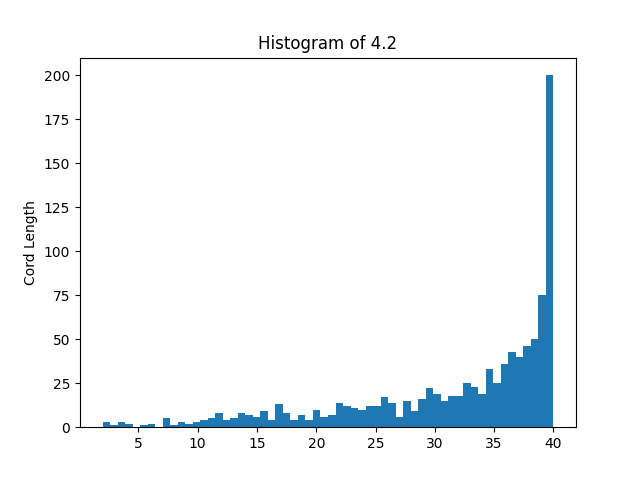
\includegraphics[scale=0.7]{Q4/Q4(2).png}
    \end{figure}
\newpage
%--------------------------------  4.3  ------------------------------------
  \subsection*{4.3}
    \begin{framed}
        For 4.3, it is similar to 4.2 with a slight difference. Instead of determining a direction, we pick a random point in the circle, and then calculates its distance from the origin $(0,0)$. If the distance is within the circle as well, we regard it as our base/adjacent of the right triangle. Then we move towards calculating the opposite/perpendicular by using pythagorean theorem, multiply it by 2 to find the total length, and then store it in the list. Then we pass that list plotting functions to plot a histogram.
        \begin{enumerate}
            \item \emph{p\_to\_o(cord)}: This function simply returns the distance between the randomly chosen point and the origin $(0,0)$. It takes a tuple of cartesian cordinates as the input and returns the distance. It uses the distance formula,
                \begin{align*}
                    dist=\sqrt{x^2+y^2}
                \end{align*}
            \item \emph{random\_point(R)}: It chooses random points for cartesian cordinates $(x,y)$ between the R and -R.
            \item \emph{cal\_cord(R,pnt)}: It takes the randomly chosen point, and finds its distance from the origin, then uses it as the adjacent/base of our right-angle triangle within the circle. Then it finds the value of the opposite/perpendicular via pythagorean theorem, and returns the twice of the opposite as the cord length.
            \item \emph{find\_cords3(R)}: This function runs 1000 times while calling the \emph{random\_point(R)} function, then it checks if the distance/base lies within the circle or not. If it does, then it proceeds to find \emph{cal\_cord(R,pnt)} and store it, else it decrements the counter by 1, to discard that value and find another.
        \end{enumerate}
        We run this program for radius 20. The histogram looks quite linear.
    \end{framed}
    \lstinputlisting[firstline=74,lastline=119,language=python]{Q4.py}
    \begin{figure}[h]
        \caption{Histogram of 4.3}
        \centering
        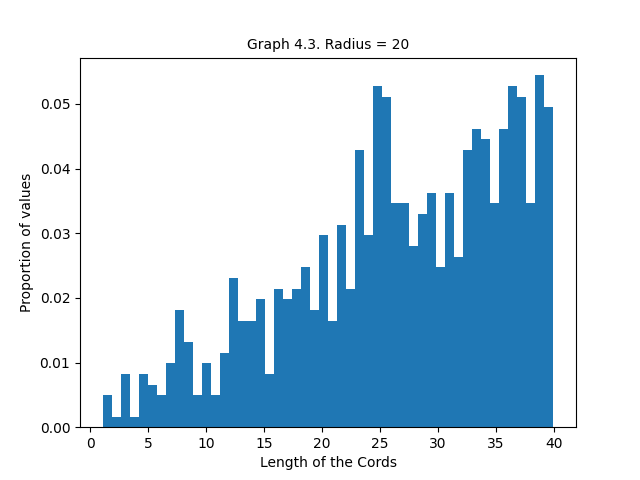
\includegraphics[scale=0.7]{Q4/Q4(3).png}
    \end{figure}
\newpage
%--------------------------------  4.3  ------------------------------------
\subsection*{4.4}
    \begin{framed}
        Out of all the distributions, I think the third approach (part 4.3) is the best to take. Its graph seems somewhat linear, which will ensure a little uniformity. As the previous graphs showed dense distribution towards the center of the circle, i.e. near the diameter, however in 4.3, the graph seems more distributed.
    \end{framed}
\end{document}